% To be \input{}'ed from the various subfolders - do not attempt to compile on
% its own!

\documentclass[10pt]{beamer}
\usepackage[T1]{fontenc}
\usepackage[utf8]{inputenc}

\graphicspath{{}{figures/}{screenshots/}}

\usetheme[progressbar=frametitle]{metropolis}
\usepackage{appendixnumberbeamer}

\usepackage{booktabs}
\usepackage[scale=2]{ccicons}

\usepackage{pgfplots}
\pgfplotsset{compat=1.12}
\usepgfplotslibrary{dateplot}

\usetikzlibrary{calc,fit,patterns}
\usepackage[absolute,overlay]{textpos}

\usepackage{xspace}
\newcommand{\themename}{\textbf{\textsc{metropolis}}\xspace}

\newcommand*{\file}[1]{\texttt{#1}}

\usepackage{xcolor}
\usepackage{listings}
\lstset{columns=fullflexible}
\lstdefinelanguage{EOL}{
morekeywords={delete,import,for,while,in,and,or,self,operation,return,def,var,throw,if,new,else,transaction,abort,
break,breakAll,continue,assert,assertError,not, switch, case, default},
sensitive=true,
morecomment=[l]{//},
morecomment=[l]{--},
morecomment=[s]{/*}{*/},
morecomment=[s]{-*}{*-},
morestring=[b]",
morestring=[b]',
showstringspaces=false
}

\lstnewenvironment{java}{\lstset{language=Java,
		frame=tb,
        tabsize=3,
        morekeywords={implies, in, result},
        basicstyle=\footnotesize,
        keywordstyle=\bfseries,
        ndkeywordstyle=\bfseries,
        commentstyle=\itshape,
		morecomment=[l]{--},
        stringstyle=\ttfamily,
		showspaces=false,
        flexiblecolumns,
        literate={->}{$\to$}{2} {--}{-$\,$-}{2} {<=}{$\le$}{2} {>=}{$\ge$}{2} {<>}{$<\,>$}{3},
        sensitive, extendedchars, texcl}}{}

\lstnewenvironment{ocl}{\lstset{language=[decorative]OCL,
	frame=tb,
	tabsize=3,
	morekeywords={implies,result,flatten,body,init,OrderedSet,Tuple,TupleType,def,attr,oclIsUndefined,oclIsInvalid,OclState,let,in},
	basicstyle=\footnotesize,
	keywordstyle=\bfseries,
	ndkeywordstyle=\bfseries,
	commentstyle=\itshape,
	stringstyle=\ttfamily,
	showspaces=false,
	flexiblecolumns,
	literate={->}{$\to$}{2} {--}{-$\,$-}{2} {<=}{$\le$}{2} {>=}{$\ge$}{2} {<>}{$<\,>$}{3},
	sensitive, extendedchars, texcl}}{}


\lstdefinelanguage{gremlin}{
morekeywords={as,def,fill,filter,groupCount,has,idx,inE,inV,is,label,length,match,outE,outV,v,values},
sensitive=true,
morecomment=[l]{//}
}

% "page cs" coordinate system
% From http://tex.stackexchange.com/questions/89588/
%
% Defining a new coordinate system for the page:
%
% --------------------------
% |(-1,1)    (0,1)    (1,1)|
% |                        |
% |(-1,0)    (0,0)    (1,0)|
% |                        |
% |(-1,-1)   (0,-1)  (1,-1)|
% --------------------------
\makeatletter
\def\parsecomma#1,#2\endparsecomma{\def\page@x{#1}\def\page@y{#2}}
\tikzdeclarecoordinatesystem{page}{
    \parsecomma#1\endparsecomma
    \pgfpointanchor{current page}{north east}
    % Save the upper right corner
    \pgf@xc=\pgf@x%
    \pgf@yc=\pgf@y%
    % save the lower left corner
    \pgfpointanchor{current page}{south west}
    \pgf@xb=\pgf@x%
    \pgf@yb=\pgf@y%
    % Transform to the correct placement
    \pgfmathparse{(\pgf@xc-\pgf@xb)/2.*\page@x+(\pgf@xc+\pgf@xb)/2.}
    \expandafter\pgf@x\expandafter=\pgfmathresult pt
    \pgfmathparse{(\pgf@yc-\pgf@yb)/2.*\page@y+(\pgf@yc+\pgf@yb)/2.}
    \expandafter\pgf@y\expandafter=\pgfmathresult pt
}
\makeatother
% Draws a grid for easier referencing of page cs values
\newcommand{\printtikzpagegrid}{
  \tiny
  \begin{tikzpicture}[overlay,remember picture,every node/.style={inner sep=.1em,draw=black!20,fill=white}]
    \foreach \x in {0,...,9} {
      \foreach \y in {0,...,9} {
        \node at (page cs:0.\x,0.\y) {};
        \node at (page cs:0.\x,-0.\y) {};
        \node at (page cs:-0.\x,0.\y) {};
        \node at (page cs:-0.\x,-0.\y) {};
      }
    }
    \node at (page cs:0,0) {0,0};
    \node at (page cs:0.5,0.5) {.5,.5};
    \node at (page cs:0.5,-0.5) {.5,-.5};
    \node at (page cs:-0.5,0.5) {-.5,.5};
    \node at (page cs:-0.5,-0.5) {-.5,-.5};
    \node at (page cs:1,1) {1,1};
    \node at (page cs:1,-1) {1,-1};
    \node at (page cs:-1,1) {-1,1};
    \node at (page cs:-1,-1) {-1,-1};
  \end{tikzpicture}
  \normalsize
}

\title{Taming Large Models\\with Hawk and NeoEMF}
%\subtitle{A modern beamer theme}
\date{MoDELS'2018, 14--19 October 2018}
\author{A. García-Domínguez, D. S. Kolovos, K. Barmpis, G. Daniel, G. Sunyé}
%\institute{Center for modern beamer themes}
% \titlegraphic{\hfill\includegraphics[height=1.5cm]{logo.pdf}}


\begin{document}

\maketitle

\pgfset{/metropolis/inner/sectionpage/.cd, none}
\section{Introduction}
\section{Hawk}
\section{NeoEMF}
\section{Mogwa\"i}

\pgfset{/metropolis/inner/sectionpage/.cd, progressbar}
\section{Wrap-up}

\begin{frame}{Summary}

  \begin{block}{Use cases}
    \begin{itemize}
    \item For fast querying with no changes to persistence: Hawk
    \begin{itemize}
    \item Make sure your models are fragmented
    \item Hawk will only re-index the changed fragments
    \end{itemize}
    \item For scalable storage with no fragmentation: NeoEMF
    \end{itemize}
  \end{block}

  \begin{block}{Feedback and contributions welcome!}
  \begin{itemize}
  \item Hawk, NeoEMF and Mogwaï are all open-source
  \item Chat with us if you have an idea for an application
  \end{itemize}
  \end{block}

\end{frame}

\begin{frame}{Hawk: project website}
  \begin{center}
    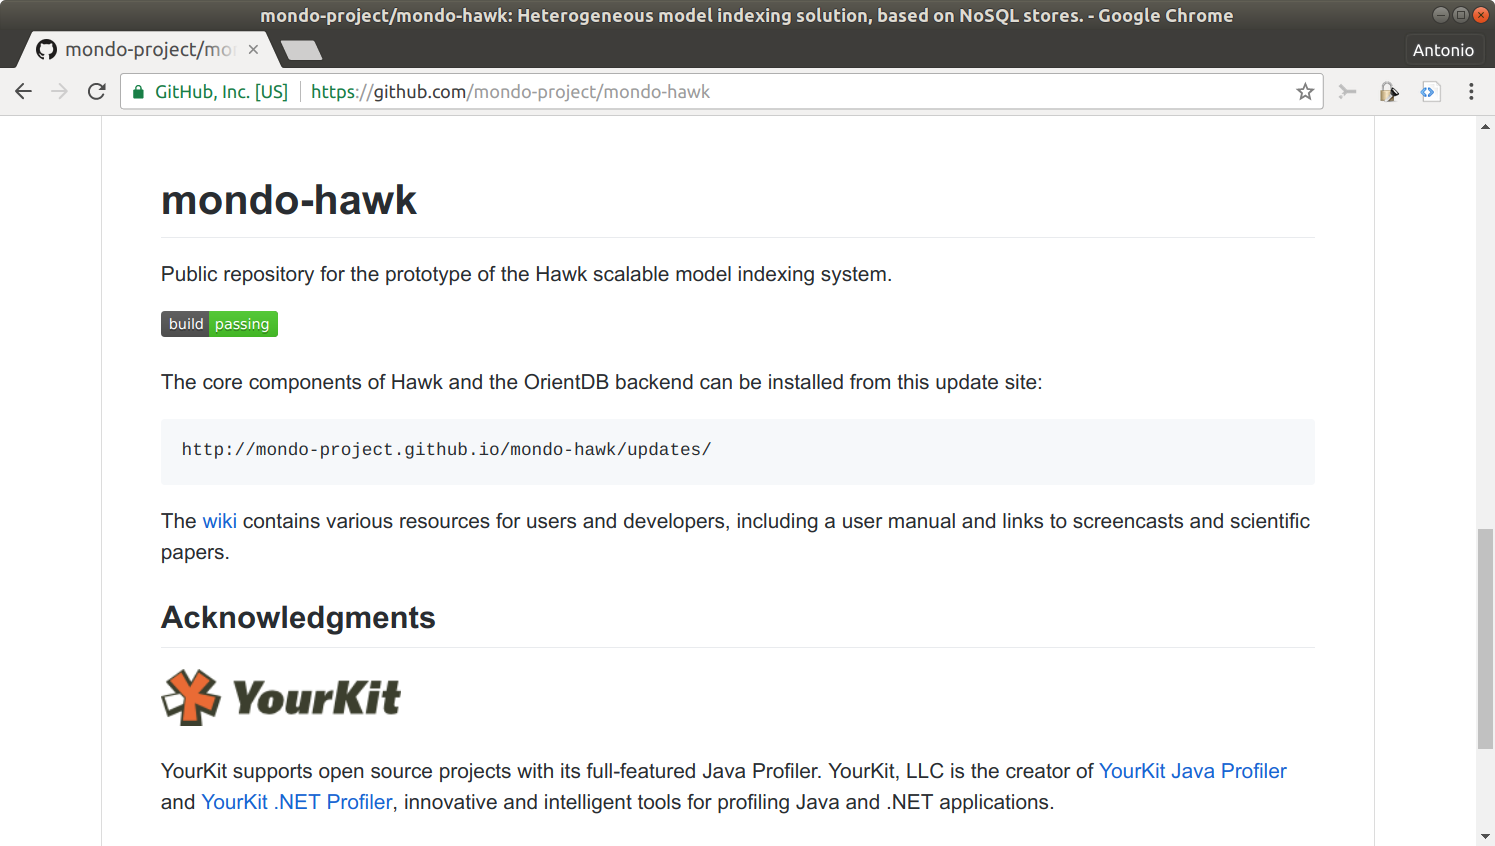
\includegraphics[width=\textwidth]{../01-hawk/figures/hawk-github}
  \end{center}

  \begin{itemize}
  \item \url{https://github.com/mondo-project/mondo-hawk}
  \item Recently accepted as Eclipse Incubator project (moving soon!)
  \end{itemize}
\end{frame}

\begin{frame}\frametitle{NeoEMF: project website}
  \begin{center}
    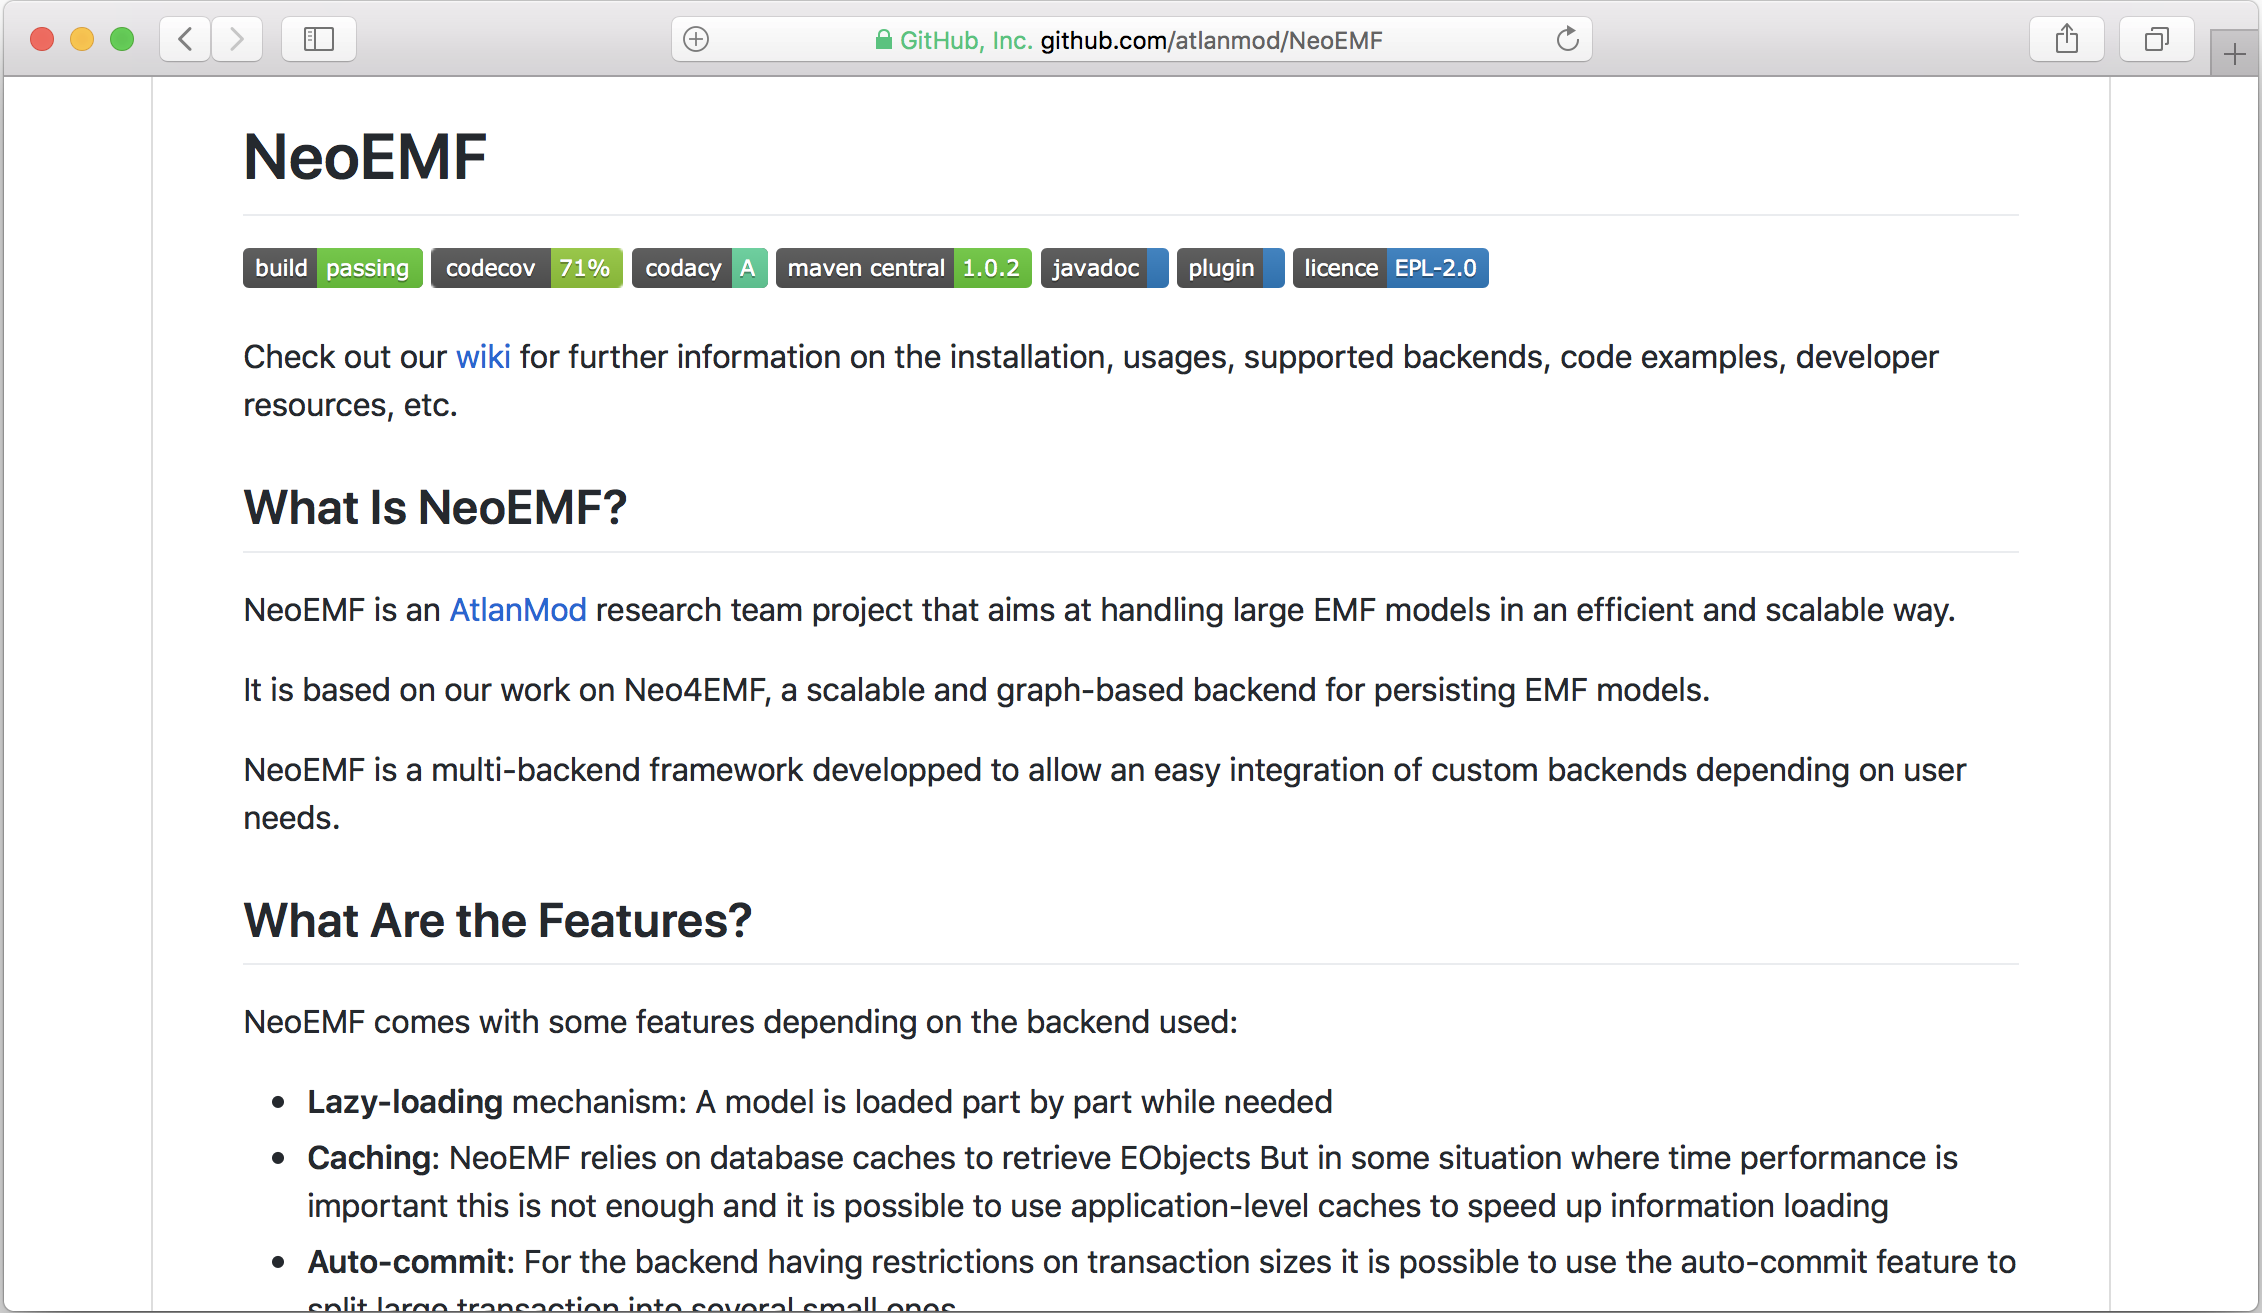
\includegraphics[width=\textwidth]{../02-neoemf/figures/neoemf-github.png}
  \end{center}
	
  \begin{itemize}
  \item \url{https://github.com/atlanmod/NeoEMF}
  \item Open source project under the Eclipse Public License 2.0
  \end{itemize}
\end{frame}

\begin{frame}\frametitle{Mogwa\"i: project website}
  \begin{center}
    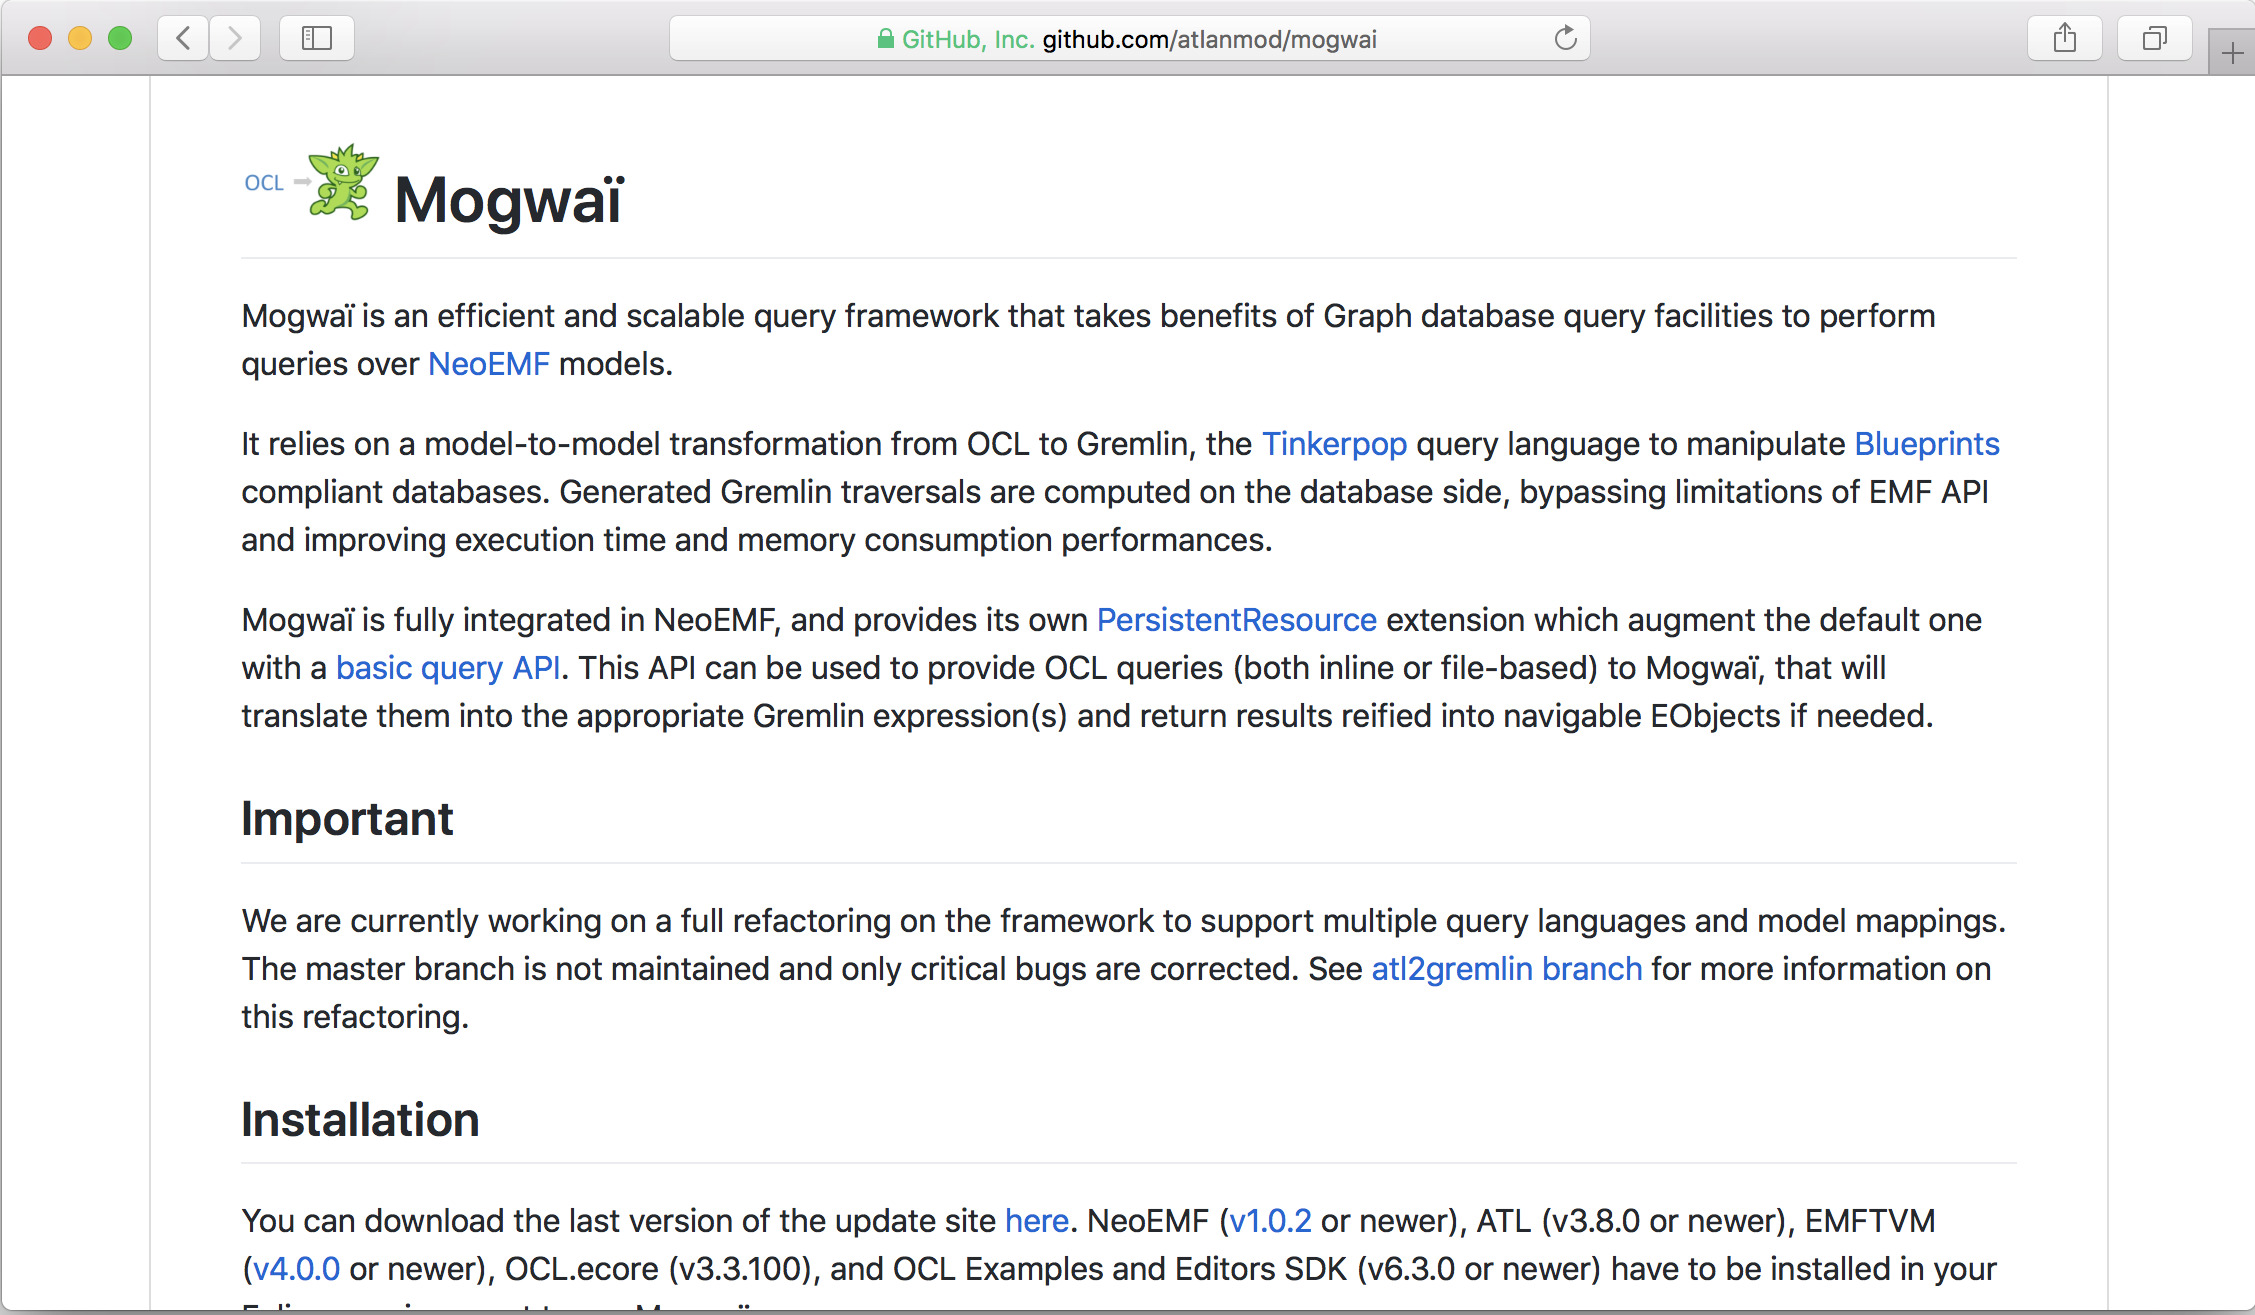
\includegraphics[width=\textwidth]{../02-neoemf/figures/mogwai-github.png}
  \end{center}
	
  \begin{itemize}
  \item \url{https://github.com/atlanmod/mogwai}
  \item Open source project under the Eclipse Public License 2.0
  \end{itemize}
\end{frame}

\begin{frame}\frametitle{Discussion}
\begin{itemize}
\item Do you plan to use the tools in your project?
\item Potential integrations with existing toolsets?
\item Any new features in mind?
\end{itemize}
\end{frame}

\appendix

{\setbeamercolor{palette primary}{fg=black, bg=yellow}
\begin{frame}[standout]
  Questions?
\end{frame}
}

%% \begin{frame}[allowframebreaks]{References}
%%   \bibliography{bibliography}
%%   \bibliographystyle{alpha}
%% \end{frame}

\end{document}
